En el circuito que se muestra en la figura de este problema tenemos: $\epsilon$ = 36 V: $R_1$ = $R_2$ = $R_3$ = 60 $\Omega$ y $R_4$ = 100 $\Omega$. Considere despreciable la resistencia interna de la batería. De las afirmaciones siguientes, señale las que son correctas:
\begin{enumerate}
    \item $R_1$, $R_2$ y $R_3$ están conectadas en paralelo.
    \item La resistencia total del circuito vale 120 $\Omega$.
    \item La lectura del amperímetro $A_1$ es 0.30 $A$.
    \item El voltaje entre $A$ y $B$ vale 6.0 V.
    \item La lectura del amperímetro $A_2$, es 0.10 A.
\end{enumerate}

\begin{figure}[H]
    \centering
    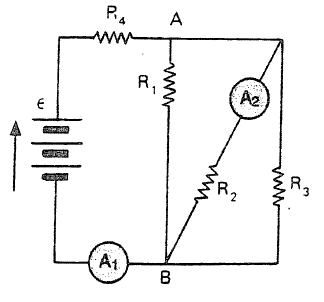
\includegraphics[width=0.5\linewidth]{enunciados/figuras/fig_alvarenga_p1005_8.png}
    \caption{Alvarenga p1005 - Ejercicio 8}
\end{figure}